% Problem and Data Description -- handbook section 3

\subsection{Problem formulation}
\label{subsec:problem-and-data-1}
% Required: Real-world motivation; input; output; prediction unit; mathematical formulation when appropriate; main difficulties.

Automated garment recognition underpins catalogue tagging, visual search and stock auditing in
online retail, where a product photograph must be routed to a category without a human in the
loop. Fashion-MNIST \cite{xiao2017fashion} is the standard small benchmark for this setting,
cheap enough to train many architectures under one protocol.

The task is single-label image classification, and the prediction unit is one image. The input is
a grayscale image $x \in \mathbb{R}^{1 \times 28 \times 28}$ and the output is one of $C = 10$
garment classes. Every model implements a function $f_\theta$ returning raw logits
$z = f_\theta(x) \in \mathbb{R}^{C}$, from which the prediction is
$\hat{y} = \arg\max_{i} z_i$. Training minimises the cross-entropy between the logits and the
true label $y$ over the training set $\mathcal{D}$:

\begin{equation}
    \mathcal{L}(\theta) = -\frac{1}{|\mathcal{D}|} \sum_{(x, y) \in \mathcal{D}}
    \log \frac{\exp(z_y)}{\sum_{i=1}^{C} \exp(z_i)}.
    \label{eq:cross-entropy}
\end{equation}

The softmax of Equation~\ref{eq:cross-entropy} is folded into the loss, so no model applies an
explicit softmax before it.

Two difficulties dominate. The four upper-body garments share a silhouette that survives poorly
at $28 \times 28$ grayscale, which Section~\ref{subsec:problem-and-data-3} shows is measurable
before any training. And because the comparison itself is the object of study, every difference
in score must trace to the architecture rather than to the data, the split or the tuning budget,
which constrains the design far more than the classification task does.

\subsection{Dataset description}
\label{subsec:problem-and-data-2}
% Required: Source, version, license; collection and labeling process if known; sample counts and annotations; class or target distribution; storage size and formats; bias and limitations.

Fashion-MNIST was released by Zalando Research \cite{xiao2017fashion} as a drop-in replacement
for MNIST, under the MIT licence. It is obtained through
\texttt{torchvision.datasets.FashionMNIST}, which downloads the four original IDX binary files,
roughly 30~MB uncompressed. The images are centred $28 \times 28$ grayscale thumbnails from
Zalando's product catalogue, labelled by the catalogue category of the article, so the labels
come from the retailer rather than from crowd workers.

The corpus holds 70{,}000 images, 60{,}000 in the official training set and 10{,}000 in the
official test set, with exactly 6{,}000 and 1{,}000 images per class respectively. The class
distribution is therefore uniform by construction, as Figure~\ref{fig:class-distribution}
confirms, and the max-to-min per-class ratio is $1.000$. No imbalance correction is required, and
accuracy and macro-F1 are not distorted by class priors.

\begin{figure}[H]
    \centering
    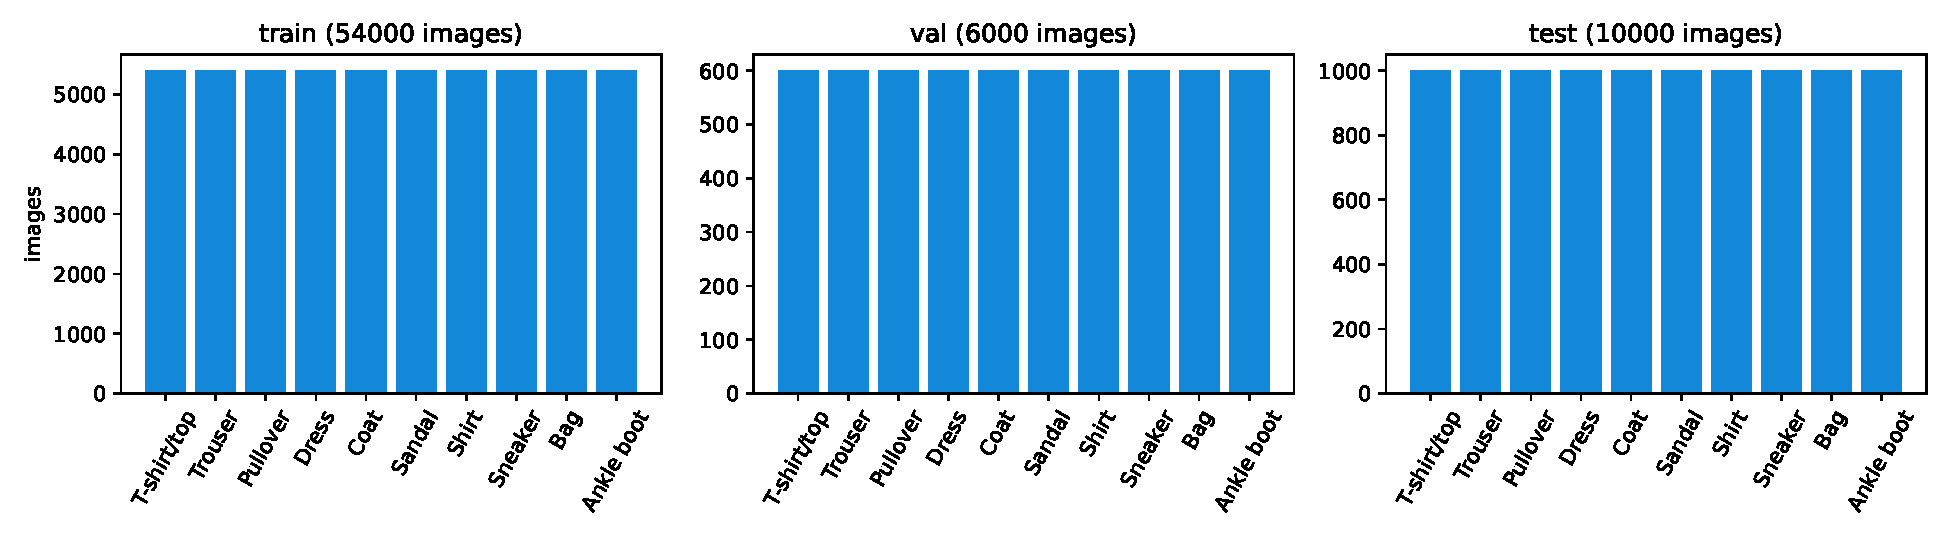
\includegraphics[width=0.8\textwidth]{images/class_distribution.pdf}
    \caption{Images per class in each subset.}
    \label{fig:class-distribution}
\end{figure}

Three limitations bound what these results can claim. The images are grayscale, square and
centred, so the models never face colour, clutter, occlusion or scale variation. The resolution
discards the fabric texture and stitching that distinguish a shirt from a coat in a real
catalogue. And the labels follow one retailer's merchandising taxonomy, in which the boundary
between a pullover, a coat and a shirt is a commercial convention rather than a visual fact, so
part of the residual error is irreducible.

\subsection{Exploratory data analysis}
\label{subsec:problem-and-data-3}
% Required: Task-appropriate analysis; the assignment chapter lists the required items.
% Also required: Section 13: EDA must include at least class distribution, input size, imbalance analysis, and representative samples.

Every image has the same input size, one channel of $28 \times 28$ \texttt{uint8} pixels, so no
resizing or padding is needed. Half of all training pixels are exactly zero and the garment is
centred, so much of the 784 flattened features carries no signal.
Figure~\ref{fig:samples} shows the variation within each class: footwear and bags are
distinctive, while the upper-body garments share an outline.

\begin{figure}[H]
    \centering
    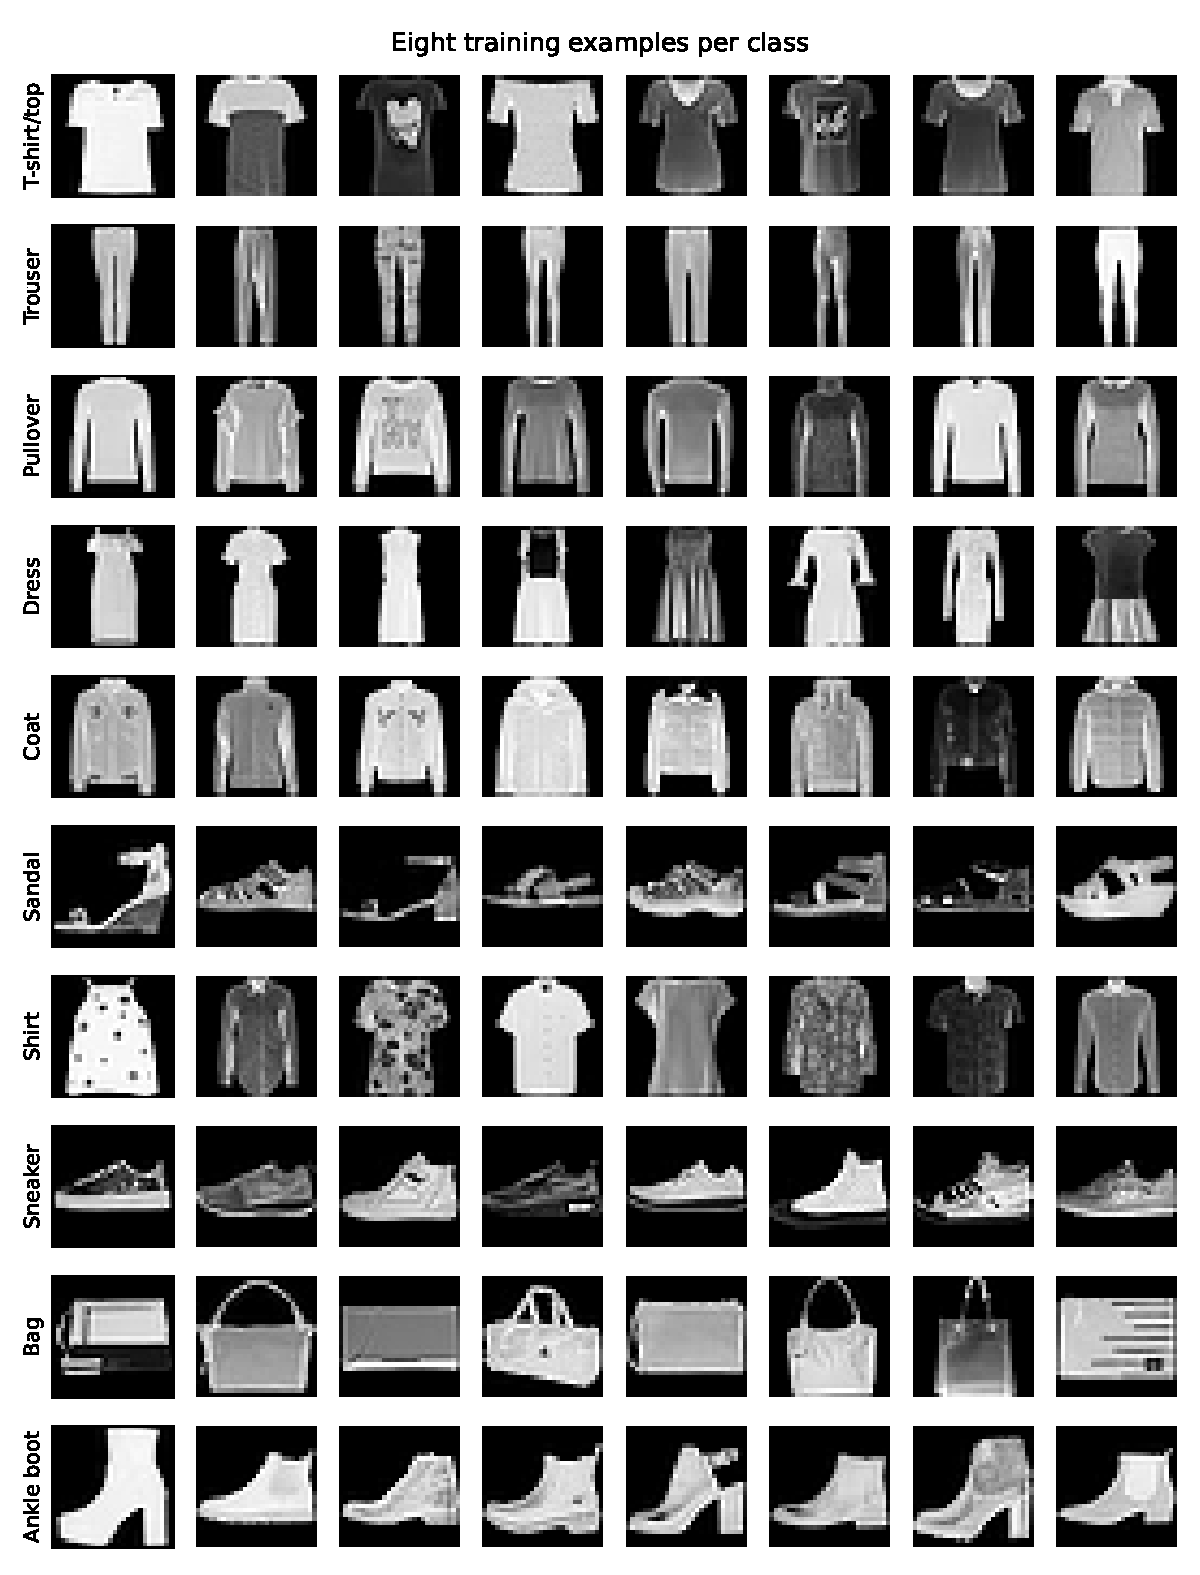
\includegraphics[width=0.85\textwidth]{images/sample_grid.pdf}
    \caption{Eight training examples per class.}
    \label{fig:samples}
\end{figure}

Class overlap is measurable before any model is trained. Cosine similarity between class mean
images exceeds $0.98$ for Coat/Shirt, Pullover/Coat and Pullover/Shirt, and a nearest-class-mean
classifier on raw pixels reaches $68.4\%$ validation accuracy with per-class recall from $0.220$
for Shirt to $0.872$ for Ankle boot. Figure~\ref{fig:overlap} reports both, and they isolate the
same cluster: a floor the trained models must clear, and a prediction of where they will fail
that Section~\ref{subsec:results-5} confirms.

\begin{figure}[H]
    \centering
    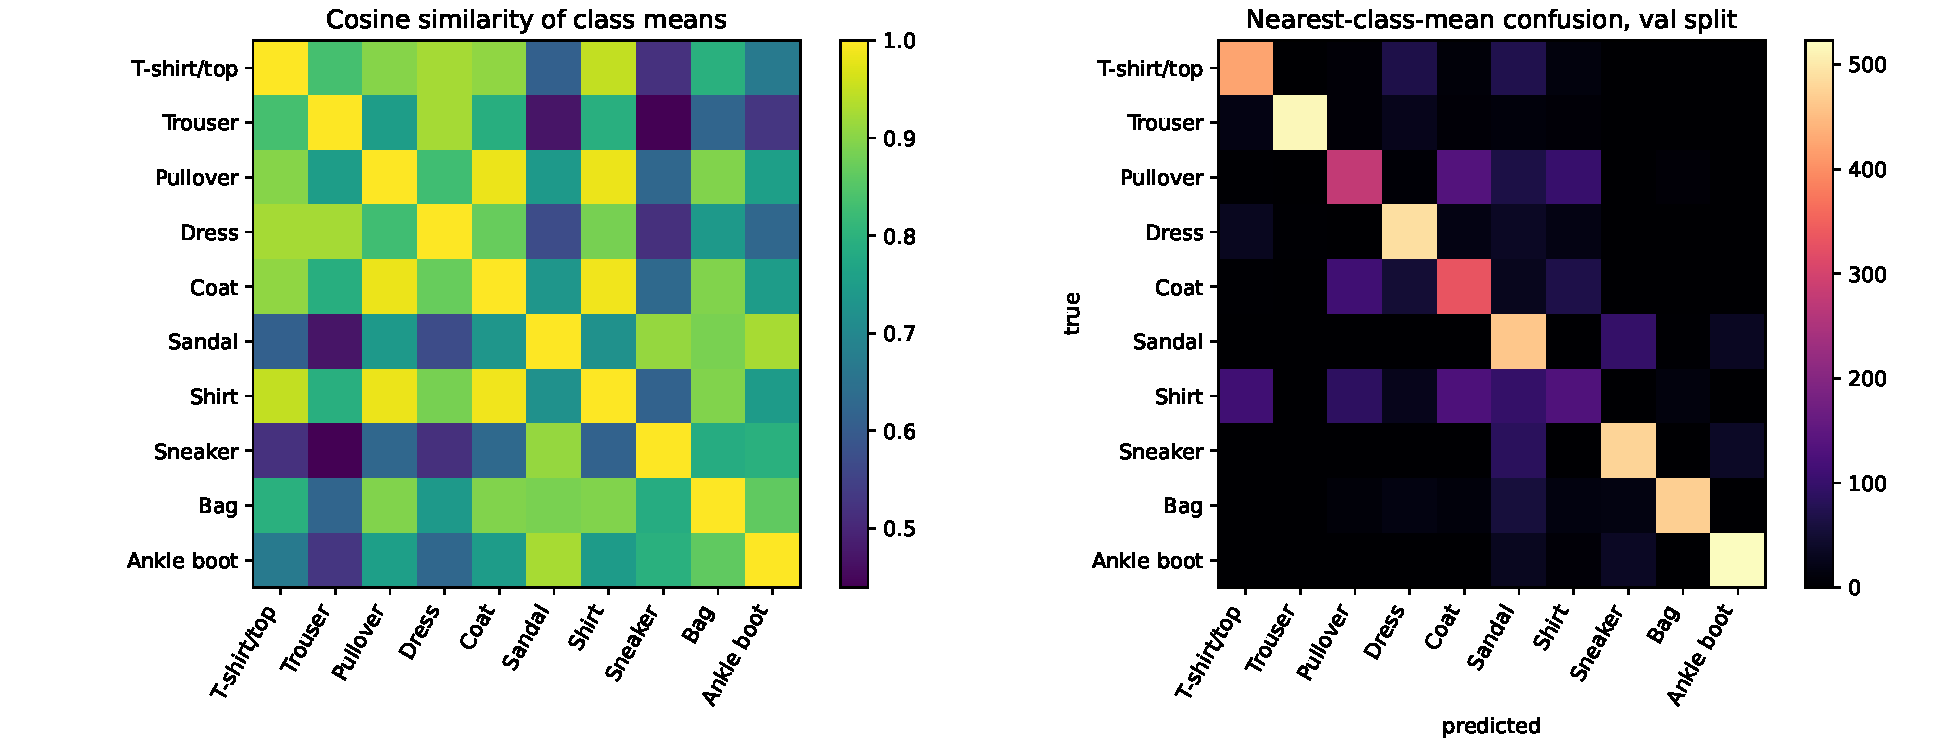
\includegraphics[width=0.95\textwidth]{images/class_similarity.pdf}
    \caption{Class mean similarity, left, and the nearest-class-mean confusion matrix, right.}
    \label{fig:overlap}
\end{figure}

The flattened view is highly redundant: ten principal components explain $72.1\%$ of pixel
variance and one hundred explain $91.4\%$. Pixel correlation falls from $0.747$ at a distance of
one pixel to $0.159$ at ten and $0.093$ at twenty. That local structure is what a convolution
exploits and a flattened view discards, a concrete reason to expect the architectures to
separate.

The same image also supports three sequence views, used by the recurrent and Transformer models:
rows and columns give 28 timesteps of 28 features, $4 \times 4$ patches give 49 tokens of 16.
Figure~\ref{fig:sequences} shows how unevenly each spreads its signal. No row falls below a
quarter of peak signal, against one column and three patch tokens, so patch tokenisation
concentrates background into a few weak tokens while rows and columns spread it across every
step.

\begin{figure}[H]
    \centering
    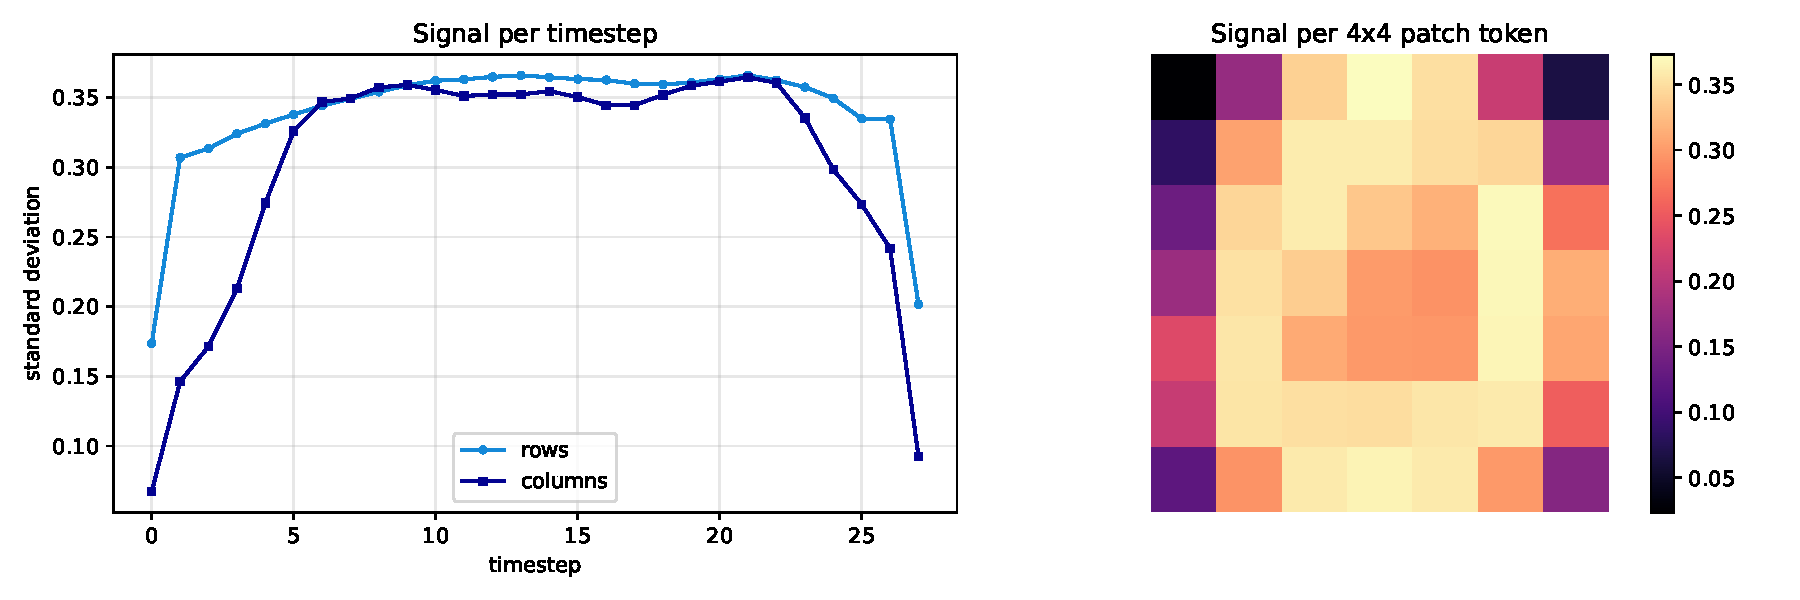
\includegraphics[width=0.95\textwidth]{images/sequence_profiles.pdf}
    \caption{Signal per timestep, and per $4 \times 4$ patch token.}
    \label{fig:sequences}
\end{figure}

\subsection{Data splitting}
\label{subsec:problem-and-data-4}
% Required: Train, validation and test; official or custom split; seed; stratification; split unit; leakage prevention; subset selection rules if any.

The official test set of 10{,}000 images is held out untouched. The official 60{,}000 training
images are split once with \texttt{train\_test\_split} at seed $0$, stratified by class, giving
the sizes in Table~\ref{tab:splits}. The split unit is the image, which is also the prediction
unit, and the images are independent product photographs, so no group structure can leak across
the boundary.

\begin{table}[H]
\centering
\caption{Split sizes.}
\label{tab:splits}
\begin{tabular}{lrr}
\hline
\textbf{Subset} & \textbf{Images} & \textbf{Per class} \\
\hline
Train      & 54{,}000 & 5{,}400 \\
Validation &  6{,}000 &   600 \\
Test       & 10{,}000 & 1{,}000 \\
\hline
\end{tabular}
\end{table}

The indices are generated once and committed, and every model loads the same file, so the split
is identical across architectures, seeds and machines. Two rules prevent leakage. Normalization
statistics are computed on the training split alone and recorded with each run, never recomputed
from the data a model is evaluated on. The test split is read only after model selection has
concluded, and once per configuration, so it never participates in any decision.

\subsection{Preprocessing}
\label{subsec:problem-and-data-5}
% Required: Cleaning; resize, normalization, tokenization, padding; augmentation; invalid annotation handling; input tensor shapes; one example batch after preprocessing.

The corpus needs no cleaning: every image is complete, every label is a valid class index, and
there are no invalid annotations to handle. No resizing or padding is applied, since the input
size is already uniform.

Images are converted to \texttt{float32} in $[0, 1]$ and standardised with the training-split
mean $\mu = 0.2858$ and standard deviation $\sigma = 0.3529$, so the network input is
$(x/255 - \mu)/\sigma$. Augmentation applies to the training loader only: a random
$28 \times 28$ crop after 2 pixels of edge padding, then a horizontal flip with probability
$0.5$. Validation and test loaders stay deterministic. The sequence models receive the same
normalised tensor and reshape it internally, to $28 \times 28$ for rows and $49 \times 16$ for
patch tokens, so tokenisation never changes the pixels.

A batch leaving the training loader is a pair of tensors: images of shape
$(128, 1, 28, 28)$ in \texttt{float32} spanning $[-0.810, 2.024]$, and labels of shape $(128)$ in
\texttt{int64} spanning $[0, 9]$. The observed range is consistent with standardisation, since
$(0 - \mu)/\sigma = -0.810$ is the value of a black pixel and $(1 - \mu)/\sigma = 2.024$ that of
a white one.
